\chapter{Path Planning}

\textbf{Author: Fabian Kleinrad} 

A crucial part of autonomy in robotics are means for planning ahead movements in a cooperative manner with the environment. Means to accomplish this are so called path planning algorithms. This chapter is going to focus on exploring the different kind of approaches to path planning and evaluate which approach is most fitting to be used in a real-time, high-dimensional use case present in the Autumn project.


\section{Algorithm Variants}

The problem of finding an optimal path between two points is an old one.
The first proposed solution was the Dijkstra's Algorithm. However with steadily evolving computer science the challenges to be master by such Algorithms got harder and harder. That's the reason why over the last years the simple principle of the Dijkstra Algorithm has branched out specializing and excelling in certain real world applications.
\footcite{Pan2020}

\subsection{Sampling-based Algoritms}

In motion planning Sampling-based Algorithms can be differentiated to other kinds of approaches, by the way they explore their environment. Sampling-based Algorithms such as the Probabilistic Road Map Algorithm or the Rapidly exploring Random Tree use a random point in their reference space and expand in that direction. This random point is considered a sample.

\subsection{Multiple-Query and Single-Query}

The term Multiple-Query refers, in connection with path planning Algorithms, to the feasibility of deriving variety of different paths, without the need of rerunning the algorithm. In Contrast Single-Query Algorithms are only able to compute one path at a time.\newline
Use cases for Multiple-Query Algorithms would be unchanging environments. The reason for that, by generating an extensive grid of connections to be able to calculate a multitude of different start/goal combinations  more computational time is needed.\newline
Single-Query approaches focus on performance instead of reuse-ability, which makes them ideal for dynamic domains. 
\footcite{Bekris2003}
\footcite{stackexchangeMultiSingleQuery2019}

\section{PRM}

Probabilistic RoadMap is a path planning algorithm tailored to multi-query application. It is considered one of the most influential sampling-based path planning algorithms. 

The algorithm can be broken down into two phases. The first phase, which is referred to as the pre-processing phase, starts with an empty graph. At first it samples n random points and adds them to a set of vertices, if they are located in space free from obstacles. After constructing a set of n vertices, it attempts connections between a random vertex and it's neighboring nodes in a predefined radius. This connecting of to vertices is realized with a simple straight line connection. All collision free connections between vertices and their respective neighbors are added to a set of edges. The result of this pre-processing phase is a roadmap, with the number of sampled points determining the quality of to be calculated paths. 
\footcite{Karaman2011}

Upon finishing the initial construction phase of a roadmap, like the one depicted in figure 8.1, start/goal combinations can be processed. 
The actual path finding in the generated graph is handled by other non-sampling-based path finding methods such as A*.\newline
With the PRM focusing on a multi-query approach it is possible to calculate a arbitrary number of different paths without the need to construct a new graph.

\begin{figure}[h]
	\centering
	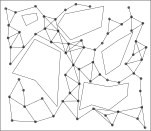
\includegraphics[width=0.8\linewidth]{img/PRMRoadmap}
	\caption{Example of a roadmap in two dimensional space constructed by the PRM algorithm.}
	\label{fig:path_planning_prm}
\end{figure}

\section{RRT Algorithm}

Rapidly exploring random tree is a path planning algorithm, that can be categorized as sampling-based and single-query. In the field of sampling-based path finding algorithms is it considered together with the PRM the most influential. RRT works by constructing a tree of possible trajectories. Therefore it is first required to define an initial vertex, much like a root. After each following iteration a random sample is taken from the space that is considered free from obstacles. After generating a random vertex, the nearest neighboring point in the tree is search for. The closest node is than used as a pivot point and a new vertex is constructed a predefined distance away from the nearest node in the direction of the random sample. Thereafter it is attempted to connect the new vertex with the nearest. If this straight-line connection can exits without colliding with obstacles it is added to the set of edges. This procedure is depicted in figure 8.2. The algorithm end when a new node is within the predefined distance away from the goal point. 
\footcite{Karaman2011}

The name rapidly exploring random tree stems from the tree like structure constructed, like the one you can see in figure 8.2, when exploring spaces This approach to path planning makes it possible to explore rapidly changing environments efficiently.


\begin{figure}[h]
	\centering
	\includegraphics[width=0.8\linewidth]{img/rrtIteration}
	\caption{Visualization of the first two iterations (a), (b) when an rrt algorithm is exploring a simple 2d space with an obstacle present. D referring to the predefined distance between vertices.\footcite{Zammit2018}}
	\label{fig:path_planning_rrt}
\end{figure}

\section{A* Algorithm}

\section{Comparison RRT with PRM and A*}

\section{RRT* Algorithm}

\subsection{Improvements to RRT}

\subsection{Implementation in Autumn}

\section{Other RRT Variants}

\subsection{RT-RRT}

\subsection{Smart-RRT}
